\documentclass[a4paper, notitlepage]{report} % type of document
\usepackage[T1]{fontenc}      % font encoding
\usepackage[utf8]{inputenc}   % sepcial chars from keyboard
\usepackage[english]{babel}   % document language
\usepackage{amsmath}          % math symbols
\usepackage{graphicx}		  % images
\usepackage{wrapfig}          % wrapped figures
\usepackage{subfig}           % subfigures
\usepackage{caption}          % required by subfig 
\usepackage{subcaption}       % captions in subfigures
\usepackage{siunitx}
\usepackage{physics}

\graphicspath{{./imgs/}}

\usepackage{geometry}
\geometry{
	a4paper,
	total={170mm,257mm},
	left=20mm,
	top=20mm,
}

\usepackage[backend = biber, style=numeric]{biblatex}         % bibliograpy


\addbibresource{summary.bib}
\title{Collective Behaviors of Interacting Active Brownian Particles: Simulations and Analysis}
\author{Candidate: Niccolò Picchiarelli \\
External Supervisor: Prof. Stefano Palagi\footnote{The BioRobotics Institute, Sant'Anna School of Advanced Studies -- Pisa}\\
Internal Supervisor: Prof. Riccardo Mannella}

\begin{document}
	\maketitle
	\textbf{Introduction.}
	\emph{Active Matter} is a term that refers to systems, both at macroscopic and microscopic scales, both natural and artificial, that consist of many independent and interacting \emph{agents}. 
	These active units can consume energy from the environment or an internal source to convert it to work and movement. 
	Such systems show peculiar individual and collective behaviors, due to the interactions that may occur between active units and to their intrinsic far-from-equilibrium nature \cite{menon_active_2010, ramaswamy_active_2017}.
	% qui ho modificato per riferirsi più in generale ad active units e non solo active particles
	Self-phoretic Janus micro-particles are a class of \emph{active particles} that convert chemical energy into self-propulsion, creating a gradient in the surrounding fluid that makes them move with a preferred direction.
	These particles are a model system for active matter, and they have been used to study collective behaviors \cite{bechinger_active_2016}.
	They have been modelled as Active Brownian Particles (ABPs), adding a deterministic self-propulsion along a given direction to classic Brownian motion.
	% aggiungi qualcosa sulle interazioni che di solito vengono usate in questi modelli
	The ABPs model stood out for its simplicity and capability of showing interesting collective dynamics.
	Literature has studied what happens when interactions are added to this model, such as excluded-volume interaction, which avoids superpositions between particles, and long-range central potentials interactions.
	%%% TOGLIEREI L'EQUAZIONE, NON MI SEMBRA UTILE
	% This model is , combined in the equations (2D)
	% \begin{equation}
	% 	\dot{x} = v \cos{\theta} + \sqrt{2D_t}\dd{W_x} , \quad \dot{y} = v \sin{\theta} + \sqrt{2D_t}\dd{W_y}, \quad \dot{\theta} = \sqrt{2D_r}\dd{W_{\theta}}
	% \end{equation}
	% where $\dd{W}$ is the derivative of a zero mean, unit variance Wiener process.
	
	%%% TOGLIEREI TUTTA QUESTA PARTE, NON MI SEMBRA UTILE
	% It is possible to show that a model like this can mimic the features of a real system of active particles \citeauthor{bechinger_active_2016}, leading the way to the discoveries of new properties of active matter, that can be used both to understand the ongoing physics behind natural systems and to create new technologies based upon such features.
	% The aim of CELLOIDS, the project inside of which this work has taken place, is to build a micro-scale intelligent robotic system utilizing self-diffusio-phoretic Janus spheres enclosed inside phospholipids GUVs (Giant Unilamellar Vesicles).
	% Janus spheres are micromotors with an inert hemispheres and a catalytic one, that, catalyzing the decomposition of some fuel, create a gradient in the product concentration field, hence causing a phoretic flow around them that makes them move with a preferred propulsion direction.
	% Under certain assumptions such micromotors behave as Active Brownian particles, showing fascinating collective motions.
	
	The objective of this thesis work is to build a minimal yet descriptive model, a simulation framework and a set of analysis tools to investigate the emergence of different collective behaviors in active particles systems.
	
	\textbf{Potential-based aligning interactions.}
	Interactions in active particles systems are classified in two categories: non-aligning, which act only on particles' positions, and aligning, which change particles' orientations and depend on them too.
	Some authors, like \citeauthor{martin-gomez_collective_2018}, showed that an aligning torque in an ABPs system can make it transition from a disordered state to an ordered one where all particles swim in the same direction \cite{martin-gomez_collective_2018}, similarly to what happens in a Vicsek model \cite{vicsek_novel_1995}.
	% questo l'ho spostato da sotto, mi sembrava avesse più senso qui
	It is known from experimental literature \cite{singh_pair_2024}, that Pt-silica Janus particles, like the ones being investigated in my host laboratory, undergo some interaction torques when close to each other. 
	Therefore, a model aiming to mimic real world behaviors needs to involve some aligning interaction.
	Starting from an existing preliminary simulation code written in the Julia language \cite{julia}, based on 2D ABPs and excluded-volume interactions, we implemented different potential-based interactions while also enhancing the speed of calculations.
	
	Our way to implement aligning interaction in an ABPs model is the main novelty of this work: instead of treating positions and orientations separately, we used central potentials like $r^{-2}$ and Lennard-Jones (LJ), applying them to an off-center position on the 2D particle, obtained starting from the center and translating of an amount $\alpha R$, where $R$ is particle's radius and $\alpha \in [-1,1]$, in the direction of self-propulsion.
	This approach is motivated by the fact that self-phoretic particles interact by their self-generated fields (hydrodynamic, chemical, electrical) that have an evident anisotropy in the self-propulsion direction.
	By changing the positions from which forces are computed and to which are applied, this model inserts a lever arm in the interaction, causing a torque to appear among particles.
	Whereas the model in \cite{martin-gomez_collective_2018} involves a non-superposition force and an explicitly aligning torque, here we show that, in the case of a purely repulsive potential, our off-centered potential-based model can show a similar transition to a flocking state.
	% in questa frase ho fatto un po' di modifiche perché non mi sembrava chiara
	Moreover, the developed model has shown to be able to qualitatively reproduce the main interaction behaviors observed in real-world experiments in my host laboratory.
	
	\textbf{Quantitative analysis of collective behaviors.}
	We studied how the global properties of the ensemble change with simulation parameters, such as the velocity, the velocity distribution, the off-center parameter $\alpha$ and the angular velocity.
	To this aim, we implemented a suite of analysis tools to study the flocking and clustering of particles, the alignment of clusters and the amount of long-range order in the ensemble.

	To better understand flocking transitions, we computed the global polarization as $P = \frac{1}{N} \abs{\sum_{k=1}^{N} e^{i \theta_k(t)}}$, where $\theta_k$ is the orientation of $k$-th particle with respect to the $x$-axis.
	Using this order parameter, we could get an insight on how a larger positive orientational coupling, as well as the presence of faster particles, can make the system polarize more and faster, while a broad distribution in angular velocity can disrupt a flocking order. %AGGIUNGI UNA FRASE SUI RISULTATI

	We know that, with potentials that allow contact between particles, such as LJ, systems like the one studied here tend to cluster.
	We then used a clustering algorithm to study how the ensemble separates into sparse particles and living crystalline lattices.
	The chosen algorithm is DBSCAN, which, with the right parameters, can mimic a common-sense definition of \emph{cluster}.
	We used maximum cluster size and cluster number to study how order in particles' positions establishes.
	Once the system is divided in clusters, we can study how the single clusters are aligned, restricting the polarization computation to the single groups.
	Using this statistic, we showed how clustering and flocking are related in most cases, with the exception of cases where a velocity distribution is present, in which the system tend to polarize even though its sparsity increases.

	The last tool that we implemented to fathom the amount of long-range order in the ensemble, is the well known pair distribution function, radial distribution function, or simply $g(r)$, which is defined \cite{hansen90a} as the average number of particles at a distance $r$ from a reference particle, normalized by the density of the system:
	$\left\langle \frac{1}{N} \sum_{i=1}^{N} \sum_{j=1}^{N}{}' \delta (\mathbf{r} - \mathbf{r}_j + \mathbf{r}_i) \right\rangle = \rho g(r)$.
	$g(r)$ made possible for us to see how a system with strongly coupled orientations is capable of developing long range order more efficiently than an ensemble with weaker orientational interaction, even when the same force is applied between particles. 
	
	%%% TOGLIEREI QUESTA FRASE GENERICA, E INCLUDEREI ESEMPI DI RISULTATI SPECIFICI SOPRA
	% With all of this, we have been able to better understand the effect of velocity, velocity distribution, orientational coupling $\alpha$ and angular velocity when a LJ potential is applied.
	
	\textbf{Inference of interactions from positional and orientational data.} 
	We developed a preliminary version of a machine learning tool, based on Graph Neural Networks, that, starting from particles positions and orientations, could predict their velocity, distinguishing self-propulsion and interactions, to infer the interaction potential, in the same spirit of \cite{ruiz-garcia_discovering_2024}.
	This tool needs more development in the data preparation part as well as in network training, since our results were not satisfying regarding the comparison between true forces and interactions learned by the GNN.

	\textbf{Conclusions.}
	%SERVONO DELLE CONCLUSIONI: HO ABBOZZATO, MODIFICA E AGGIUNGI QUALCHE RIFLESSIONE CRITICA, POTENZIALE IMPATTO DEL TUO LAVORO IN QUESTO AMBITO DI RICERCA, E PROSPETTIVE FUTURE
	We developed a model of Active Brownian Particles with aligning interactions, that can reproduce the main behaviors observed in real-world experiments.
	We implemented a suite of analysis tools to study the collective behaviors of the system, and we used them to study the effect of different parameters.
	We also developed a preliminary version of a machine learning tool to infer the interaction potential from positional data.
	This work opens the possibility for a simple yet descriptive model, that unifies aligning and not aligning interactions.
	%Some more interaction parameters could be added to reproduce the real world behaviors' variety.
	More work is needed in order to make simulations in quantitative accordance with Janus self-phoretic particles experiments.
	One step further both for the experimental purpose and modeling is making the inference more accurate: when this tool will give enough confidence in its ability to predict interaction potentials it will be used to infer potentials from experiments, making the model more accurate and complete.
	
	\begin{figure}[htp]
		\centering
		\subfloat[][]{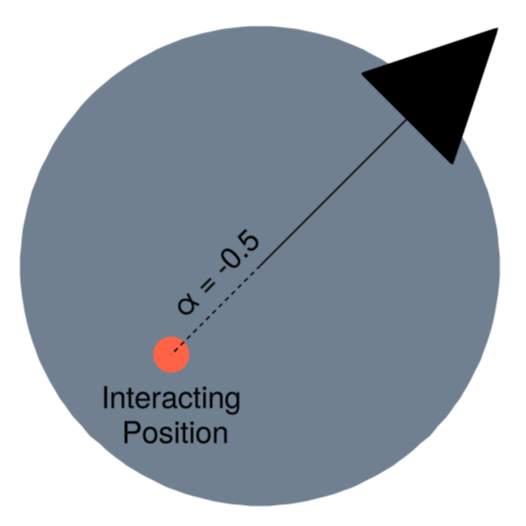
\includegraphics[width=.25\textwidth]{singpart_draw.png}}
		\subfloat[][]{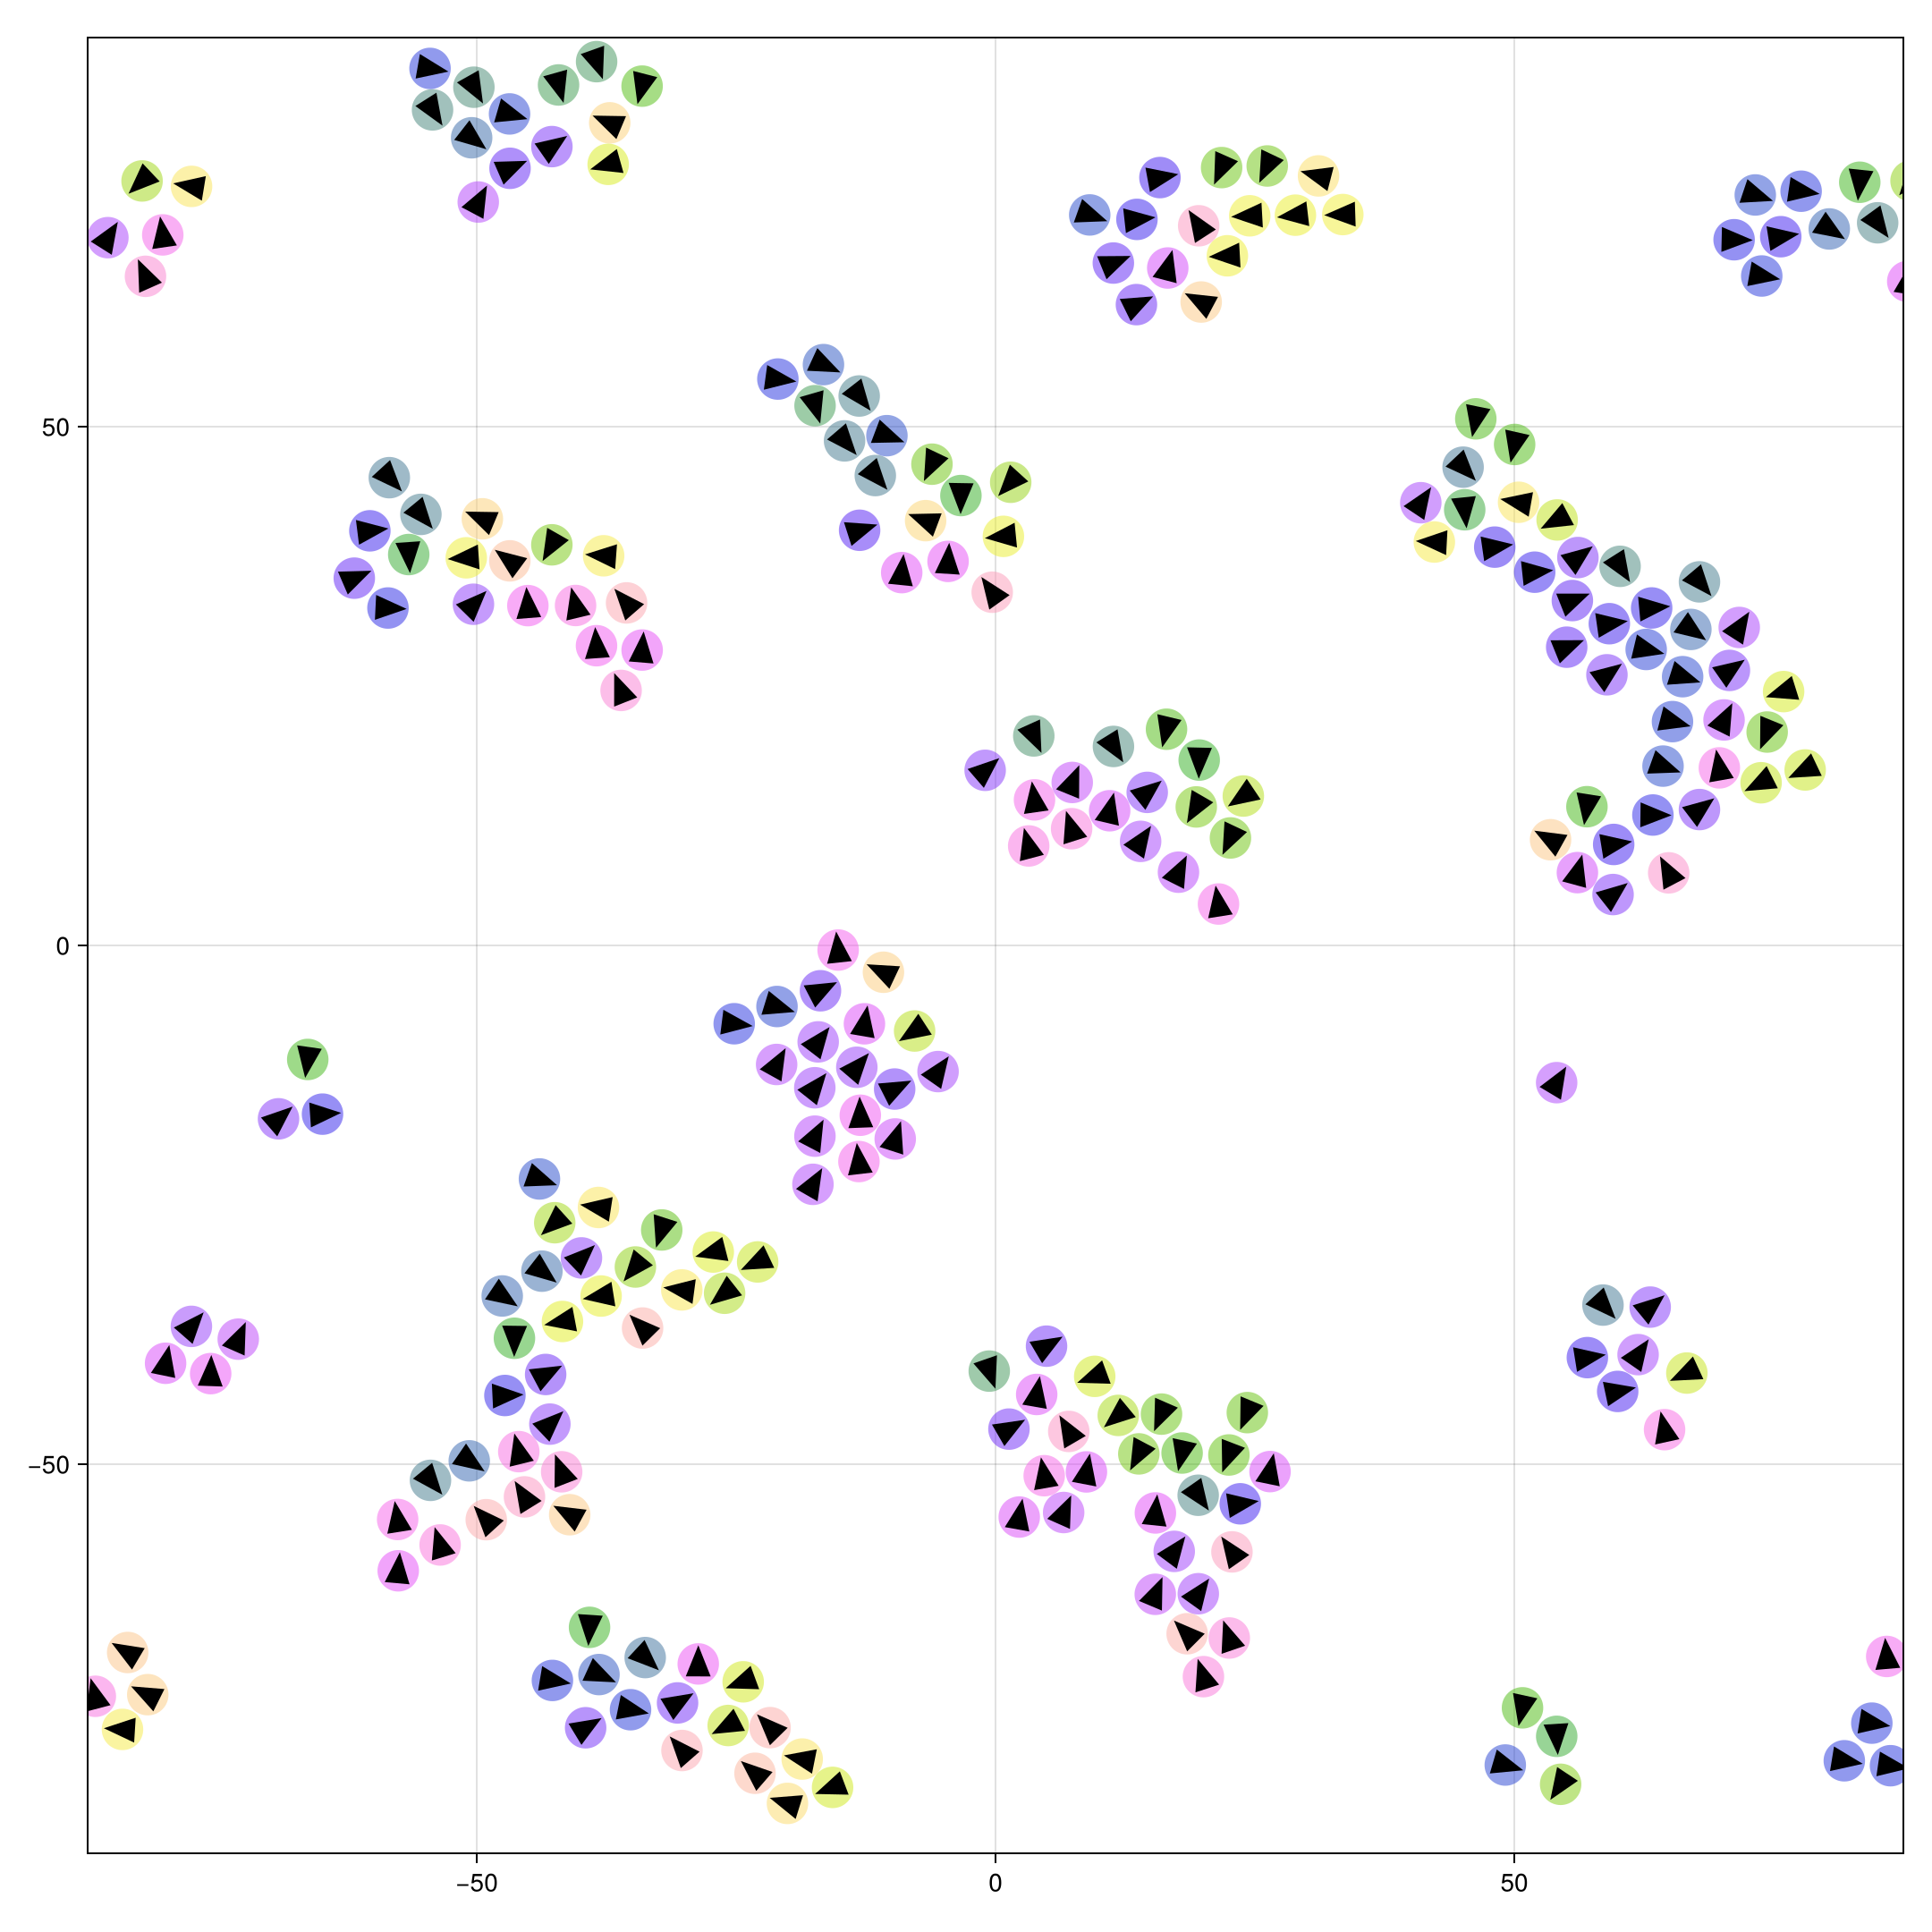
\includegraphics[width=.25\textwidth]{situa0.0_oc0.5.png}}
		\subfloat[][]{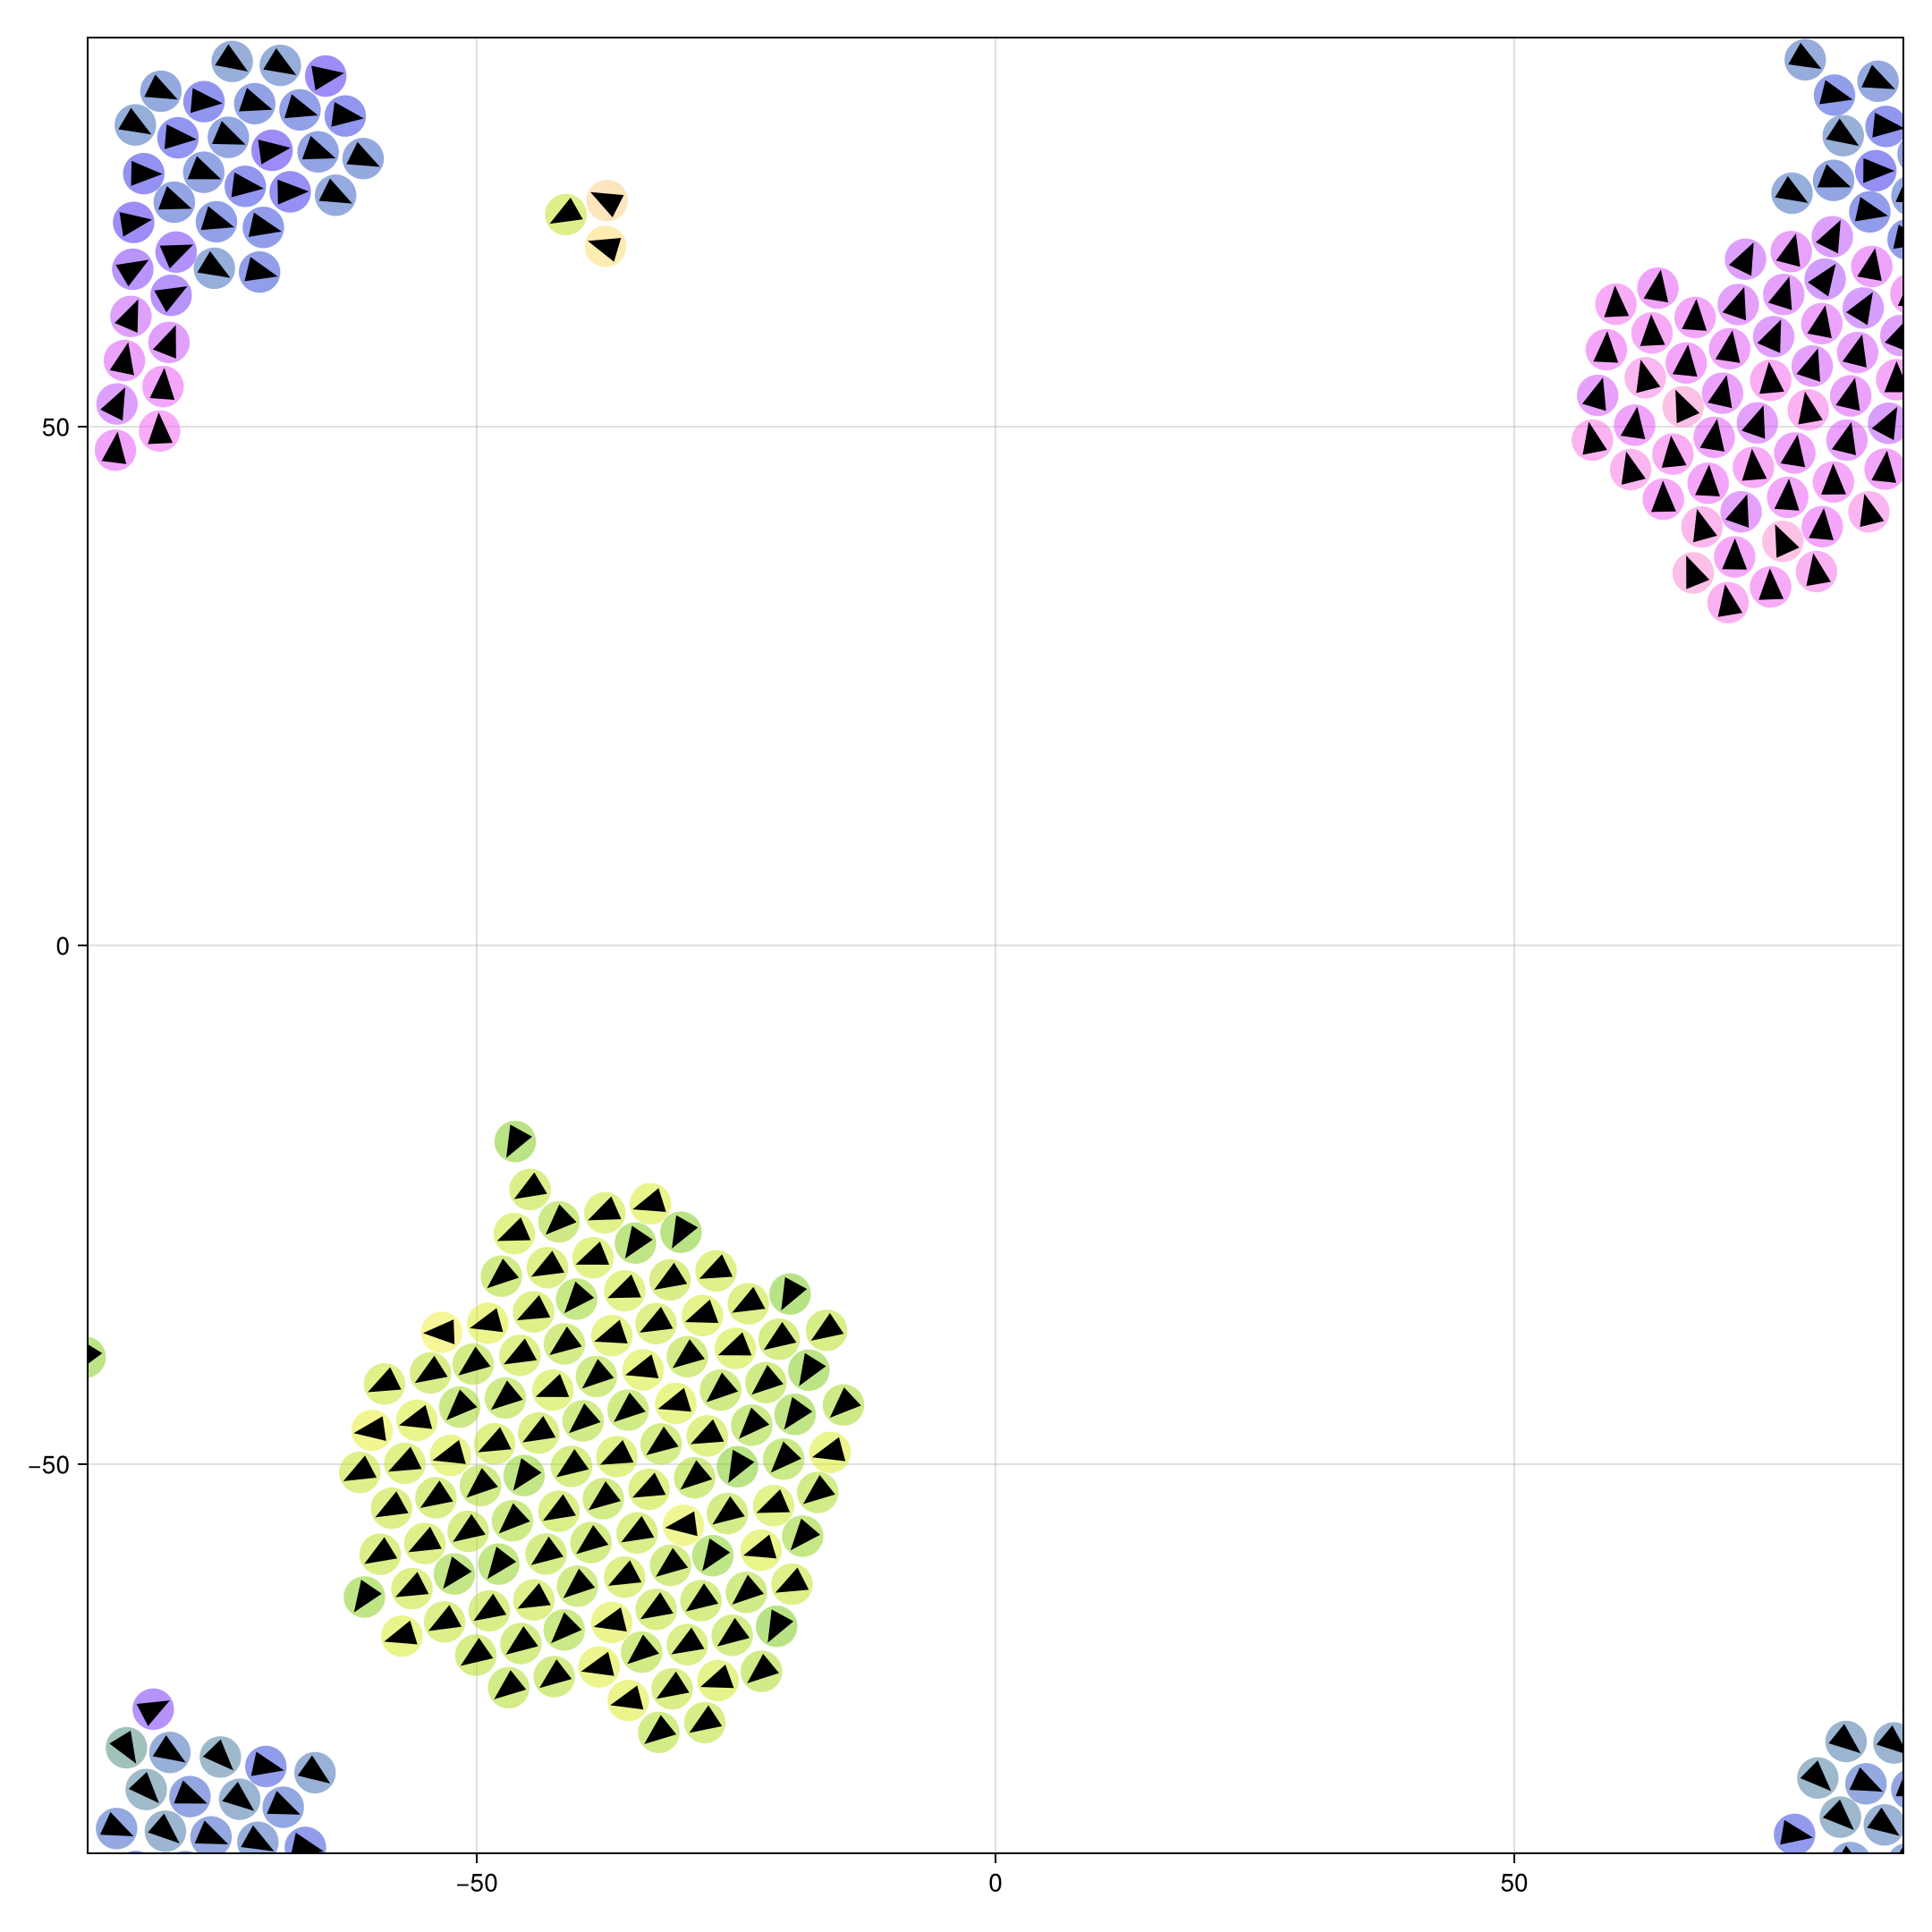
\includegraphics[width=.25\textwidth]{situa0.5.png}}
		\subfloat[][]{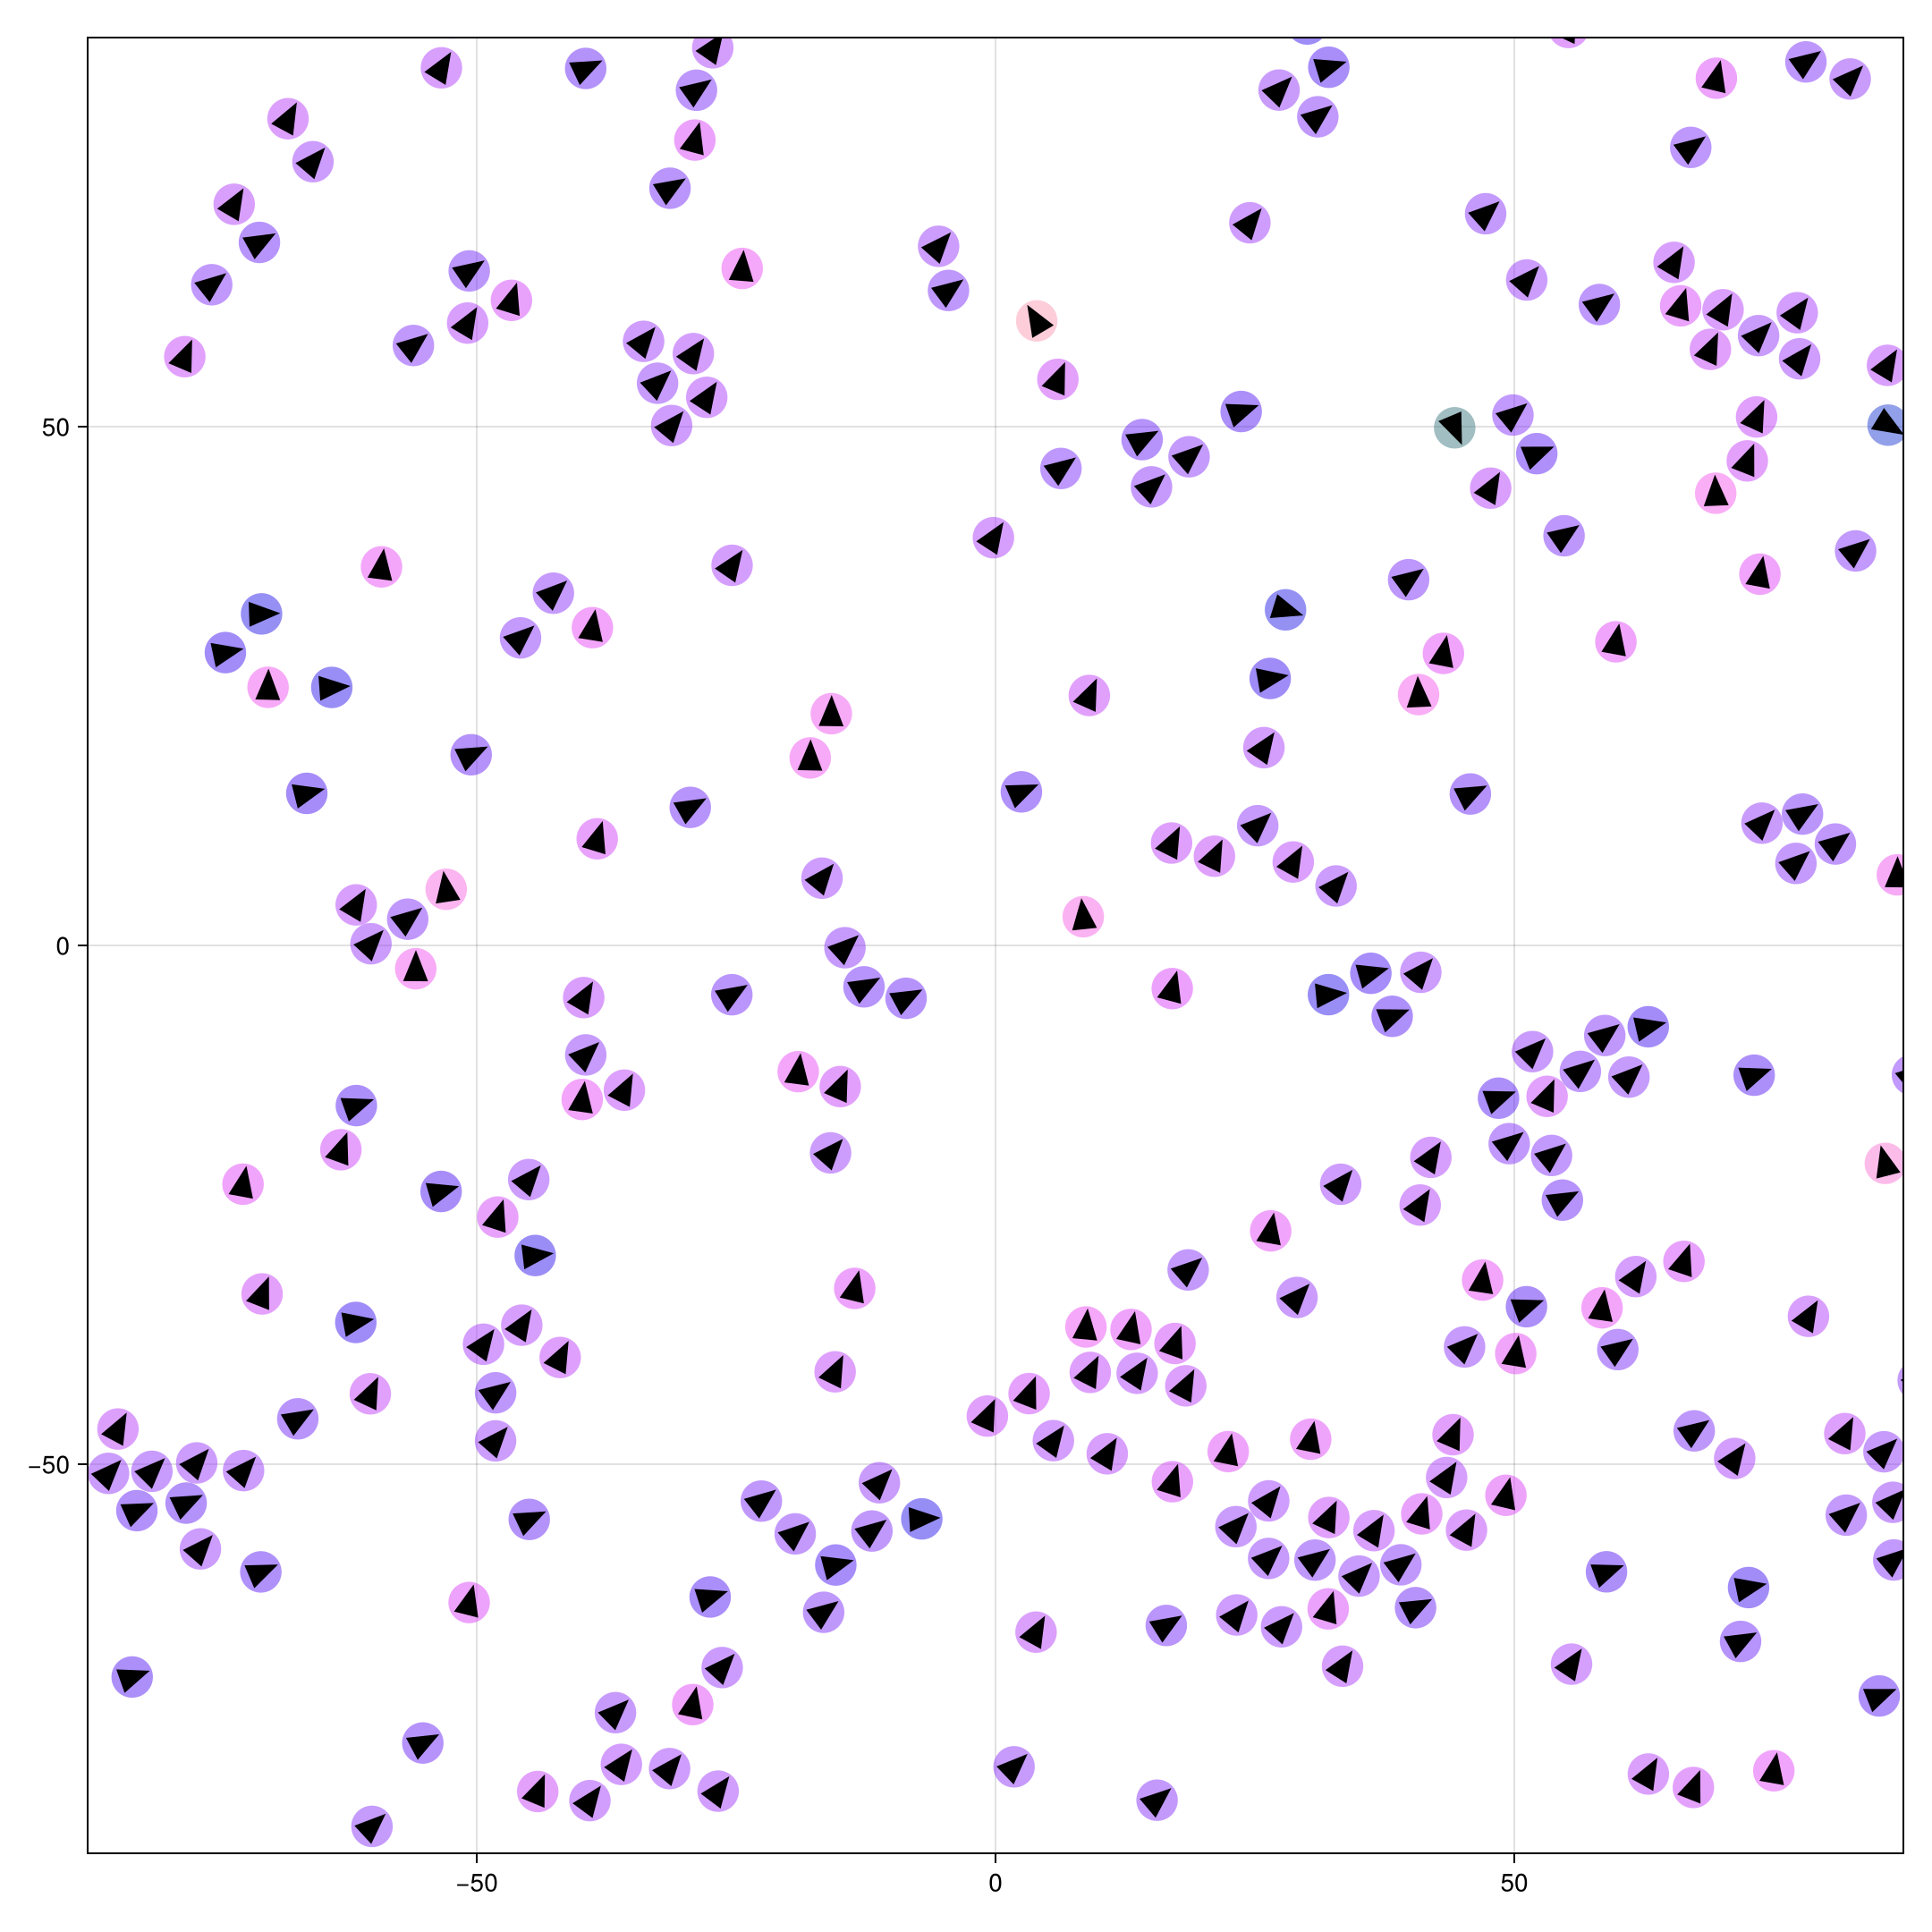
\includegraphics[width=.25\textwidth]{situa10.0.png}}
		
		\caption{(a) schematic of off-center interacting position, black arrow represents self-propulsion direction. (b-d) collective behaviors, from left to right: clustering without flocking with zero self-propulsion velocity, clustering and flocking angular velocity distribution $\mathcal{N}(\SI{0}{\radian\per\second}, \SI{0.5}{\radian\per\second})$, flocking without clustering for self-propulsion velocity distribution $\mathcal{N}(\SI{10}{\um\per\second}, \SI{10}{\um\per\second})$. All simulations are performed under a LJ potential with (b and d) $\sigma = \SI{4.}{\um}$, $\epsilon = \SI{0.1}{\pico\joule}$, (c) $\sigma = \SI{4.}{\um}$, $\epsilon = \SI{0.25}{\pico\joule}$}
	\end{figure}
	
	\printbibliography
\end{document}